
\subsection{\texorpdfstring{$\ttbar$}{h1} and\texorpdfstring{$~\ttbar$}{h2}-like background}
\label{Sec:emuSS}

The background from electrons arising from non-singularly produced W and Z bosons is estimated directly
from Monte Carlo simulation as in the 13~\TeV\ analysis.
The leptonic decay of \ttbar and $tW$ processes are generated using powheg, while the $WW$, $WZ$ and $ZZ$ are generated using pythia8.
The $Z/\gamma*\rightarrow \tau\tau$ processes are generated using amc@NLO.

All these processes are flavour-symmetric and have a branching ratio to a pair of leptons of different flavour,
$e\mu$, twice as large as the branching ratio to $e^{+}e^{-}$. This means the $e-\mu$ mass spectrum provides an
excellent control region to validate the Monte Carlo predictions for these backgrounds. This validation is described below.
%The contribution of these backgrounds to the e$^{-}$ e$^{+}$ spectrum is estimated from Monte-Carlo
%simulations after having checked that the simulations describe the sample of $e\mu$ events well.
In order to study the $e-\mu$ mass spectrum, we use the SingleMuon datasets and 'HLT\_Mu50' trigger is applied on data events.
The electron-muon events are selected such that the first object is a global muon passing the high $p_{T}$ muon identification criteria\cite{CMS-AN-2016-391},
and the second object is an electron passing the HEEP ID selection. Electron is required to have $p_{T}>35~\mathrm{GeV}$ while muon is required $p_{T}>60~\mathrm{GeV}$.
Since high energetic muons can produce bremsstrahlung and an associated super-cluster in the ECAL in the direction of the muon's
inner track, the selected muons can lead to fake electron candidates. Therefore, an electron veto is applied such that if there is
a global muon with $p_{T} > 5$ GeV within $\Delta R <0.1$ of the electron, the electron is not selected. Finally the electron and muon should have opposite sign.
The Monte Carlo samples and the cross-sections used are documented in table~\ref{tab:Z_mc-samples_1}, all scale factors have been applied to mc event.

The estimation of the multi-jet background from simulated samples is not feasible because of the small misreconstruction rate for the jets.
Instead, the multi-jet background is obtained from the same sign $e\mu$ spectrum, where the electron and muon have the same charge.
The contributions of the other SM processes (estimated from simulations) are subtracted from the data
spectrum in same sign $e\mu$ spectrum and the remaining spectrum is taken to come from multi-jet events. For the multi-jet background, the spectrum for the same sign or
opposite sign e$\mu$ pair should be the same.


The invariant mass spectrum of $e\mu$ events in data and MC spectrum are shown for both datasets in Figure \ref{fig:ttbaremu}.

%=================================================
\begin{figure}[!htb]
\begin{center}
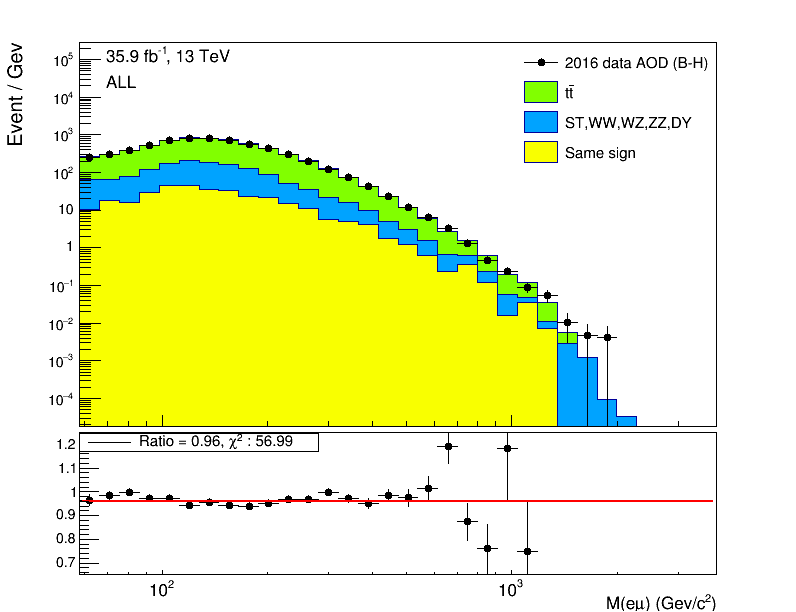
\includegraphics[angle=0,width=0.47\textwidth]{figures/Zprime/2016/bkg_ttbar/SS/hratio_M_emu1__ALL.png}
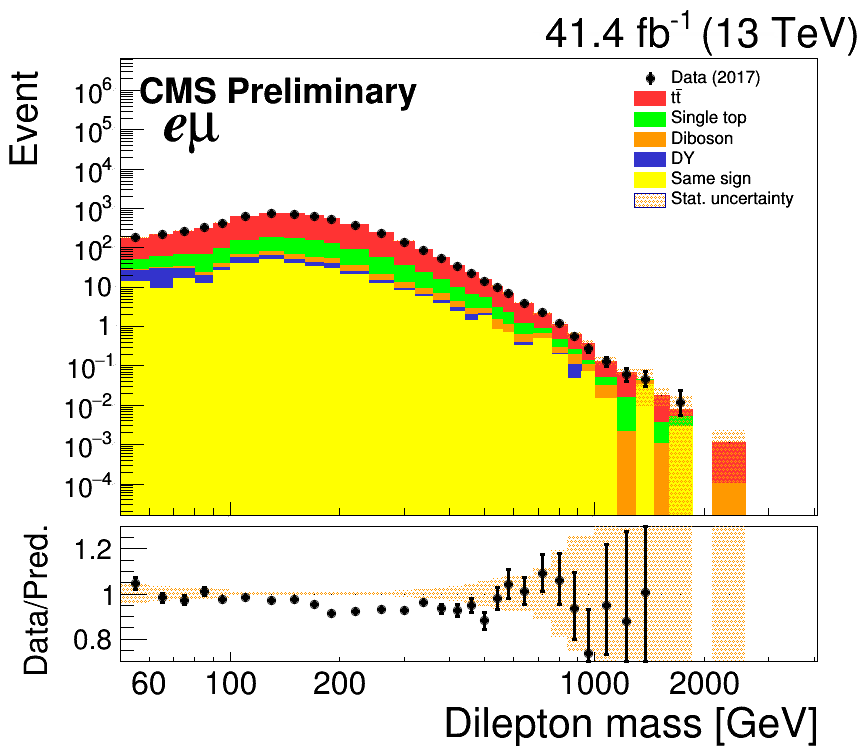
\includegraphics[angle=0,width=0.47\textwidth]{figures/Zprime/2017/bkg_ttbar/SS/ALL_hratio_M_emu_massDep.png}
\caption{Invariant mass spectra of the $e\mu$ events in data and MC for 2016 (left) and 2017 (right).}
\label{fig:ttbaremu}
\end{center}
\end{figure}
%=================================================

After having checked that the simulations describe the sample of $e\mu$ events well, the
contribution of these backgrounds to the $ee$ spectrum is estimated from Monte Carlo.
Tendency of data/MC ratio is known effect from top $p_{T}$, which is not corrected in above plot.


